\section{Implementation}
\label{sec:impl}

\subsection{Technology}
Solidity 0.8.24 with the optimizer at 200 runs, OpenZeppelin Contracts 5.0.2 \cite{openzeppelin}
(attributed), Hardhat 2.28 \cite{hardhat}, ethers v6, Node.js with Express and sql.js (SQLite in
WebAssembly) for the off chain services, and React 18 with Vite for the frontend.

\subsection{Smart contracts}
\paragraph{Creating a circle (W1).} \code{CircleFactory.createCircle(config)} makes an EIP 1167 clone of
the single \code{Circle} implementation \cite{eip1167}, calls \code{initialize} in the same transaction
(so nobody can front run the set up), and registers the clone with the vault, the draw and the
registry. \code{initialize} can run once, only when called by the factory, and rejects settings that
are invalid or would not fit the packed storage.

\paragraph{Joining (W2).} \code{join} checks the state, the join deadline, that the caller is new, that
the circle is not full and that the caller's past defaults are within the circle's limit, then pulls
the slot 1 deposit into the vault. The join that fills the circle moves it to \code{OrderDraw} and
starts the draw.

\paragraph{Drawing the order (W3).} Each member commits
$\text{keccak256}(\text{secret}\,\|\,\text{member}\,\|\,\text{circle})$, then reveals once every member has
committed or the commit window has closed. \code{finalizeDraw} may be called by anyone once everyone
revealed or the reveal window is over. Members who did not reveal are removed: one contribution of
their deposit is taken as a penalty and shared by those who revealed, the rest is refunded, and a
default is recorded. With two or more revealers the order is a Fisher Yates shuffle of the revealers
driven by the combined secrets and the hash of the block that holds the last reveal (fix S2,
Section~\ref{sec:s2}); excess deposits are refunded and round 1 starts. With fewer than two, the
circle is cancelled and everyone is refunded (when nobody revealed, no penalty is taken, bug B-1
reported by Member B).

\paragraph{Paying and settling (W4, W5).} \code{contribute} sets the member's bit in the round's paid
bitmap and pulls one contribution. \code{settleRound} is allowed once everyone paid or the deadline
(round length plus grace plus any time paused) has passed. It applies the default rules of
Section~\ref{sec:collateral}, repays the recipient's debt from the pot, refills the recipient's
deposit, credits the rest to \code{withdrawable} and starts the next round, or completes the circle.

\paragraph{Claiming and completing (W6, W7).} \code{claimPayout} zeroes the caller's credit before
transferring it (checks, effects, interactions) and is never blocked by a pause. The last settlement
takes any leftover debt from deposits, releases every deposit and records completions for members
without defaults.

\paragraph{Cancelling (W8).} The organizer may cancel while the circle is open; anyone may once the
join deadline has passed. Every deposit is refunded.

\subsection{Off chain services}
\begin{itemize}
  \item \textbf{IPFS terms store.} The organizer's browser hashes the terms, uploads them, and checks
        the returned CID (version 1, raw codec, sha2-256 \cite{multiformats}) before creating the
        circle. The same CID a real IPFS node would print is computed locally, and an optional Kubo
        node can pin the file.
  \item \textbf{Indexer and API.} Polls the logs of every known contract, applies events in block and
        log order to SQLite, detects chain resets and reorganisations by block hash, and can be deleted
        and rebuilt from events at any time. It serves circle lists, history, reputation and signed
        display names over HTTP.
  \item \textbf{Notifier.} Turns events and deadlines into in app reminders (commit and reveal due,
        payment due, payout ready, default recorded). In Stage 3 it was changed to read each active
        circle's current deadline from the chain, because a pause now extends it.
  \item \textbf{Keeper.} Reads circles from the factory, simulates \code{settleRound},
        \code{finalizeDraw} and \code{cancel}, and sends only calls that will succeed.
\end{itemize}

\subsection{Frontend}
The browser app connects MetaMask (or, on the local chain, any Hardhat test account), checks the
network, offers a faucet, and shows each circle with role chips and only the actions the contract
would accept at that moment. Every transaction goes through a tray that shows wallet confirmation,
mining and the result with its hash and gas; failed calls are decoded into plain sentences (every
revert string in the contracts has one; a Stage 3 test enforces this). Figure~\ref{fig:ui} shows an
active circle; Figures~\ref{fig:terms} and \ref{fig:offline} in Section~\ref{sec:security} show the off
chain trust checks.

\begin{figure}[H]
\centering
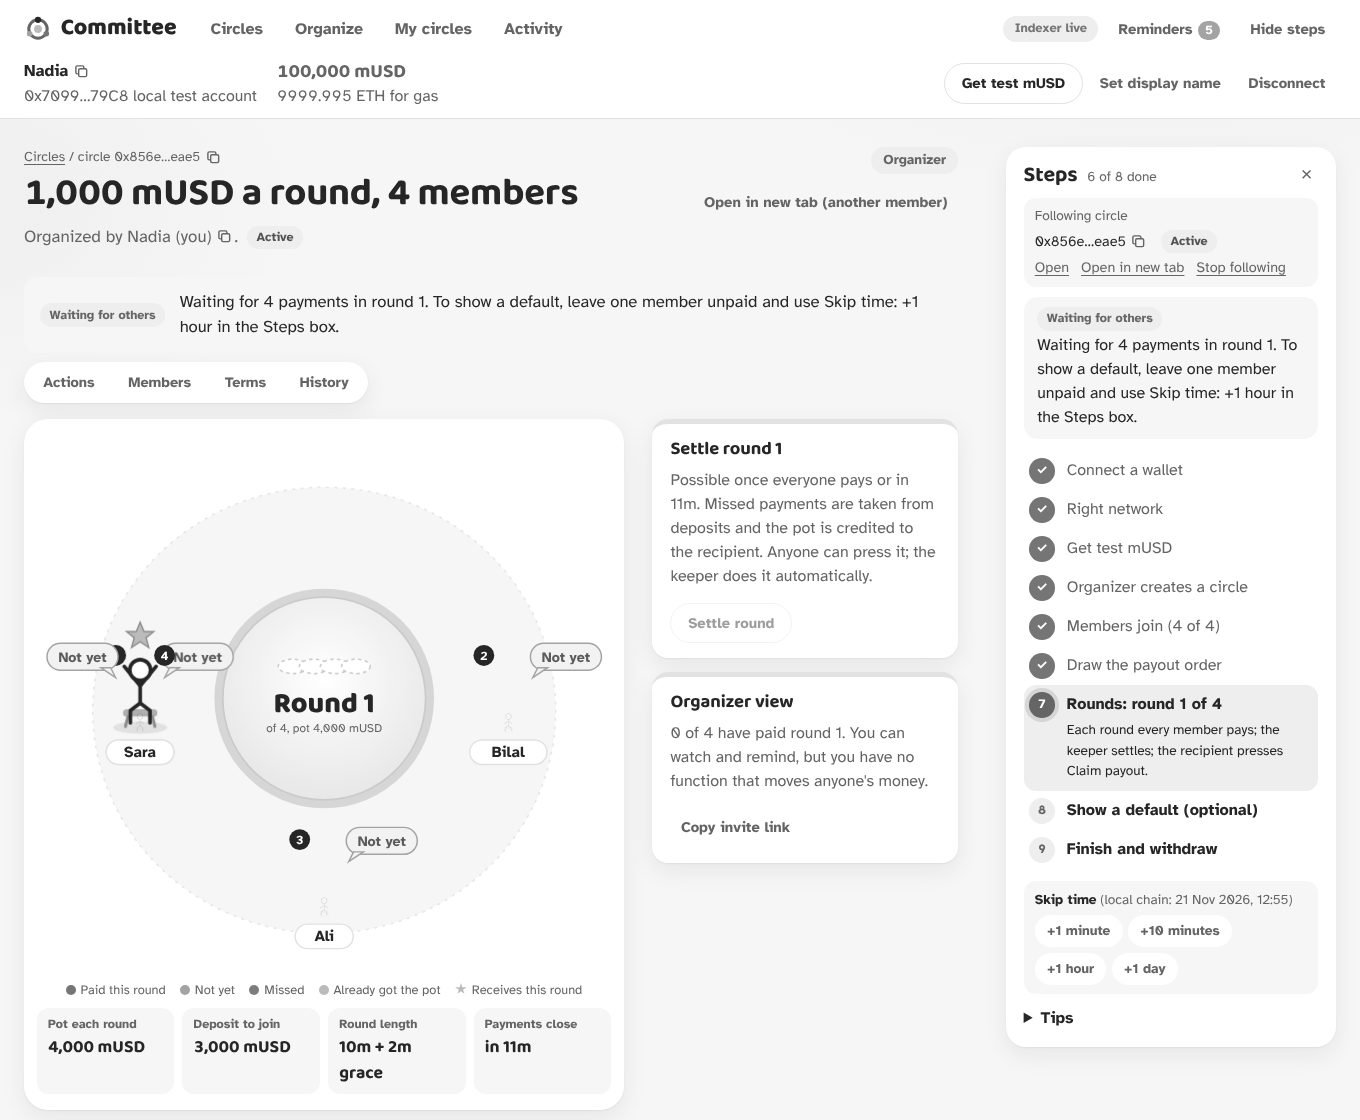
\includegraphics[width=0.86\textwidth]{figures/shot_active_round.jpg}
\caption{Organizer view of an active circle: seats in payout order, who has paid, the settle action}
\label{fig:ui}
\end{figure}

\subsection{Development workflow}
One shared repository, one member holding the code at a time. Each stage ended with a tag and a one
page handoff note in \code{docs/handoff/}, and the next member started by running the whole test
suite from that tag. Member C's rule was to change contract internals only, never function
signatures or events, so the frontend and indexer keep working; a Stage 3 test now proves this
automatically (Section~\ref{sec:abi}). Stage 3 work is on the \code{develop} branch, with one commit per optimization, fix or
document set, so each change can be measured and reviewed on its own (Appendix~\ref{app:commits}).
